\section{Hall effect}
\begin{figure*}
	\centering
	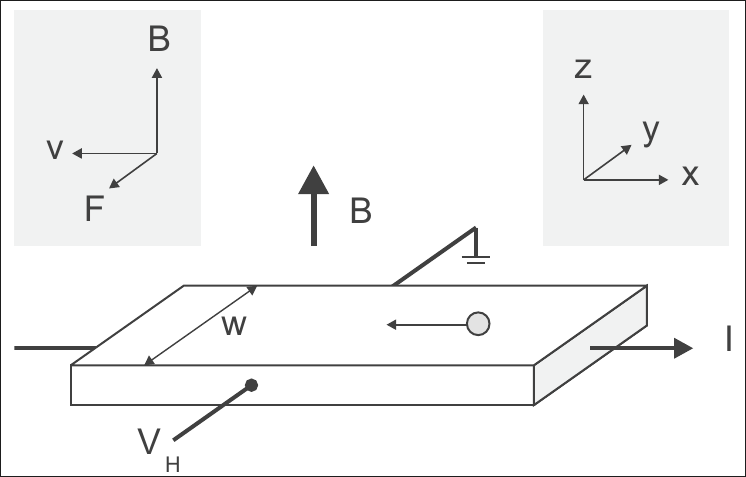
\includegraphics[width=0.8\linewidth]{../assets/hall_geometry.png}
	\caption{Schematic structure for Hall effect measurements.
		\imcite{grundmann}}
	\label{fig:hall}
\end{figure*}
The geometrical arrangement required for Hall effect measurements
is displayed in \cref{fig:hall}.
A magnetic field $\mathbf{B}=B \cdot \hat{z}$ penetrates
a semiconductor sample.
A current $\mathbf{j}$ is flowing along the $x$-direction inside the sample 
as a response to an external electric field $\mathbf{E}=E_x \cdot \hat{x}$.
Due to the magnetic force, the electrons are deflected and a current in
$y$-direction establishes until the resulting electric force in $y$-direction
fully compensates the magnetic force.
The system equilibrates for $j_y=0$.

To describe the system in detail for one majority charge carrier, one can use the 
equation of motion from relaxation time approximation:
\begin{equation}
	m^{*} \frac{\mathbf{v}}{\tau}=q(\mathbf{E}
	+\mathbf{v}\times \mathbf{B}).
\end{equation}
In this equation, $m^{*}$ is the effective mass of the charge carrier, $\mathbf{v}$ the
average electron velocity and $\tau$ the relaxation time constant.
With $\mathbf{j}=nq\mathbf{v}$ and the resistivity tensor $\hat{\rho}$, 
this vector equation can be brought into a linear transformation of the form
$\mathbf{E}=\hat{\rho}\mathbf{j}$ or more explicit:
\begin{equation}
	\label{eq:mej}
	\begin{pmatrix}
		E_{x} \\
		E_{y} \\
		E_{z}
	\end{pmatrix}
	=
	\begin{pmatrix}
		\frac{m^{*}}{\tau nq^{2}} & - \frac{B_{z}}{nq}        & 0                         \\
		\frac{B_{z}}{nq}          & \frac{m^{*}}{\tau nq^{2}} & 0                         \\
		0                         & 0                         & \frac{m^{*}}{\tau nq^{2}}
	\end{pmatrix}
	\begin{pmatrix}
		j_{x} \\
		j_{y} \\
		j_{z}
	\end{pmatrix}.
\end{equation}
The system equilibrates for $\mathbf{j} = j_x \cdot \hat{x}$ and with \cref{eq:mej}, the following
relationship holds true: $E_{y} = B_{z} / (nq) j_{x} = R_{\mathrm{H}}B_{z}j_{x}$.
This leads to an expression for the carrier density $n$ using directly measurable quantities.
\begin{align}
	R_{\mathrm{H}}&=\frac{1}{nq}=\frac{E_{y}}{j_{x}B_{z}}\\
	n&=\frac{j_{x}B_{z}}{E_{y}q}
\end{align}

Now we want to find an expression for the mobility.
\begin{equation}
	\begin{pmatrix}
		E_{x} \\
		E_{y} \\
		E_{z}
	\end{pmatrix}
	=\begin{pmatrix}
		\mu_\mathrm{H}^{-1} & -B_{z}              & 0                   \\
		B_{z}               & \mu_\mathrm{H}^{-1} & 0                   \\
		0                   & 0                   & \mu_\mathrm{H}^{-1}
	\end{pmatrix}
	\begin{pmatrix}
		v_{x} \\
		v_{y} \\
		v_{z}
	\end{pmatrix}
\end{equation}
The hall mobility in this equation is defined as $\mu_{\mathrm{H}}=\frac{q\tau}{m^{*}}$.
To see why this is useful, first, think of the limit $B_{z}\to 0$.
Then, electric field and velocity indeed follow the relation $\mathbf{v}=\mu_{\mathrm{h}}\mathbf{E}$.
Second with $\mathbf{v}=\mu_{\mathrm{h}}\mathbf{E}$ one can easily see that
$v_{x} = \mu_{\mathrm{H}}E_{x}$ and $E_{y}=B_{z}v_{x}=B_{z}\mu_{\mathrm{H}}E_{x}$.
Therefore we find the following equation for $\mu_\mathrm{H}$:
\begin{equation}
	\mu_{\mathrm{H}}=\frac{E_{y}}{B_{z}E_{x}}
\end{equation}

\subsection{Van der Pauw Method}
The Van der Pauw Method is a measuremtn technique to measure the resistivity as well as the hall coefficient.
It is possible to measure samples with nearly arbitrary flat shapes and examine it's resistivity $\rho$, 
mobility $\mu_\mathrm{H}$ as well as it's sheet carrier density $n$. 

Only samples that met the subsequent conditions can be measured with the Van der Pauw method:
\begin{itemize}
	\item The contacts are at the circumference of the sample.
	\item The contacts are sufficiently small (compared to the sample size).
	\item The sample is homogeneous and isotropic cocerning doping as well as thickness.
	\item The surface of the sampele is singly connected, i.e., the sample does not have isolated holes.
\end{itemize}
To utilize the Van der Pauw method, four ohmic contacts need to be placed on the sample.
These contacts should be as small as possible and as close as possible to the samples periphery. 
All contacts and all wires should be constructed from the same material. 

After the ohmic contacts are places, the resistivity $\rho$ can be measured.
Each contact is labeled counterclockwise with a number from 1 to 4.
The current $I_{12}$ is then defined as the positive current injected into contact one and extracted from contact two.
The voltage $V_{34}$ is given by the potential difference between contact three and four as $V_{34}=V_4-V_3$. 
With these definitions, the resistivity can be calculated as $R_{12,34}=\frac{V_{34}}{I_{12}}$. 
Van der Pauw's theorem states that the resistivity can be calculated as 
$$
\begin{align}
\rho&=\frac{\pi d}{\ln(2)} \left( \frac{R_{12,34}+R_{23,41}}{2} \right)f
\left( \frac{R_{12,34}}{R_{23,41}} \right) \\
\label{eq:hall_resistivity}\\
\frac{R_{12,34}-R_{23,41}}{R_{12,34}+R_{23,41}}&=f \, \text{arccosh}\left( \frac{\exp(\ln(2 /f))}{2} \right)
\label{eq:hall_resistivity_f}
\end{align}
$$
where $d$ is the thickness of the sample and $f$ is a correction factor that satisfies \cref{eq:hall_resistivity_f}. 
The reciprocal theorem states that the resistances obey the relation $R_{12,34}=R_{34,12}$ and $R_{12,34}=R_{21,43}$.
Therefore, we can measure the resistivity with four different contact configurations to increase measurement accuracy.

Within the Van der Pauw configuration, it is also possible to determine the Hall coefficient $R_{\mathrm{H}}$ if 
one can establish a homogeneous magnetic field $\mathbf{B}=B_{0} \hat{z}$ perpendicular to the samples surface. 
The Hall coefficient can be calculated as
$$
R_{\mathrm{H}}=\frac{d}{IB_{z}} [U_{13}(B_{z}=0)-U_{13}(B_{z}=B_{0})].
\label{eq:hall_coefficient}
$$
The difference in  \cref{eq:hall_coefficient} accounts for the Hall voltage that originates from the earths magnetic field.



